\section{More Analysis}




\subsection{Error Analysis}
\label{subsec:error_analysis}
\begin{figure}[htbp]
    \centering
 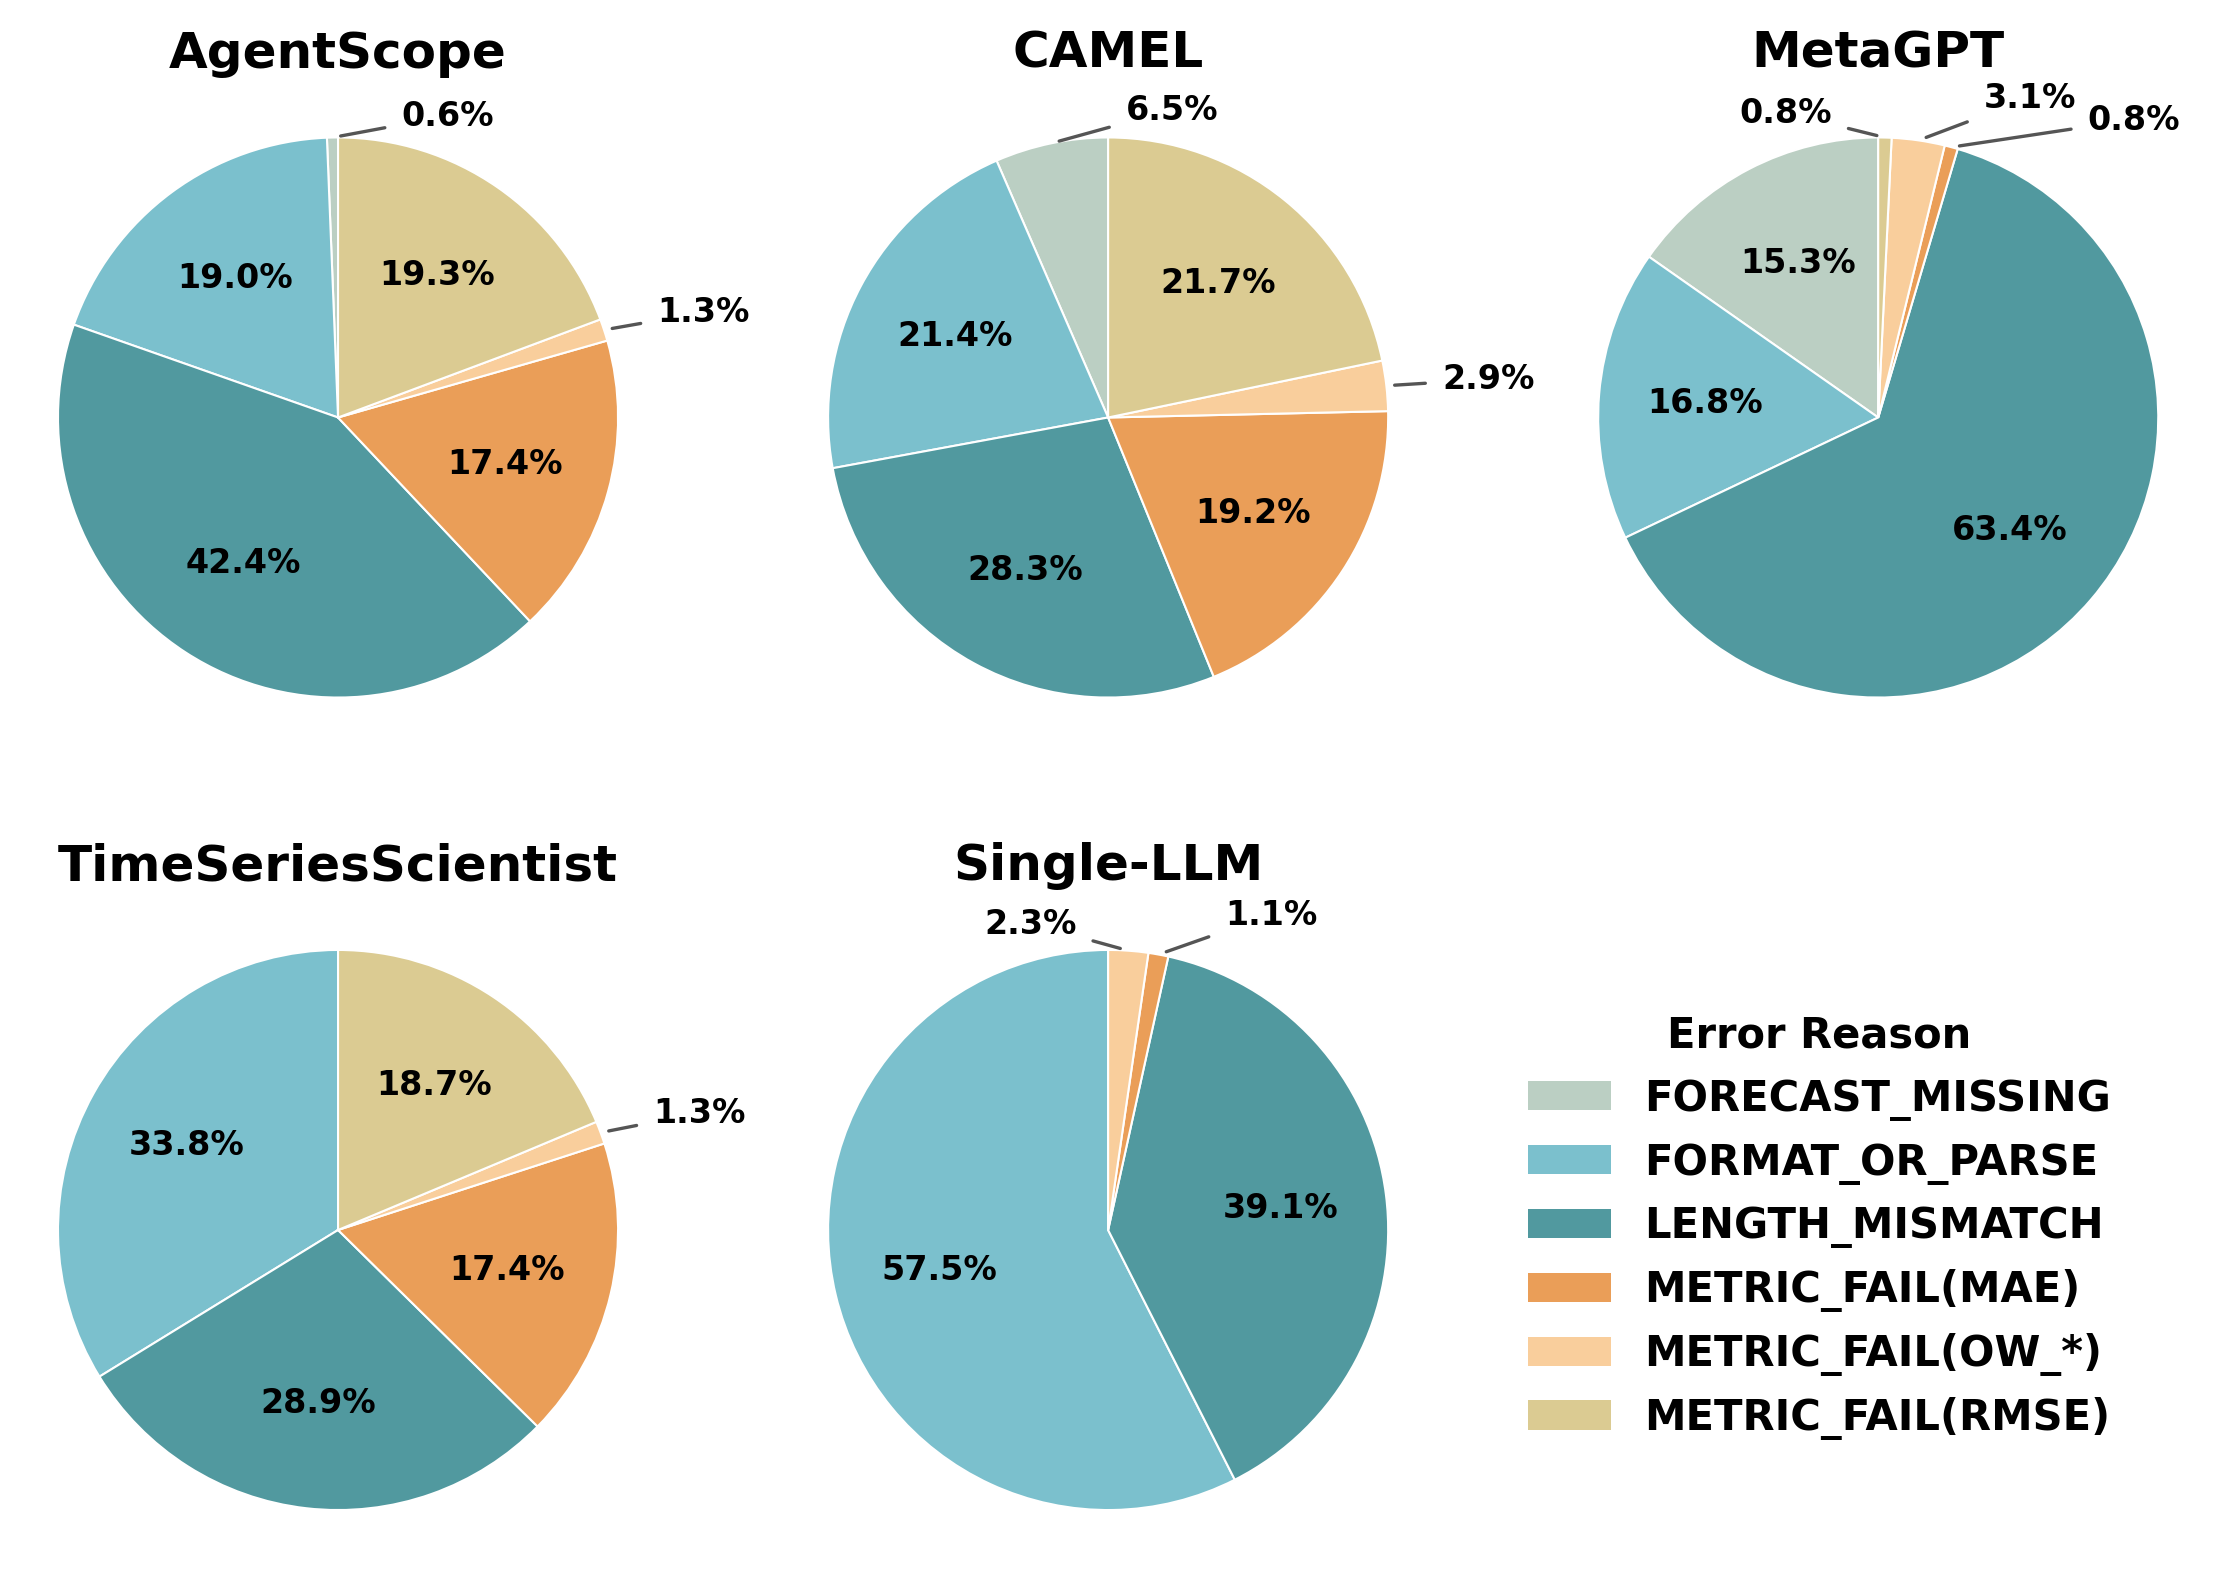
\includegraphics[width=\columnwidth]{images/error_pies_by_agent.png}
    \caption{
Distribution of error types across five agents using \texttt{gpt-4o} as the base LLM, aggregated over all datasets and tasks.
Each pie chart corresponds to an agent and shows the proportion of different failure modes.
}

    \label{fig:error_type_distribution}
\end{figure}
Figure~\ref{fig:error_type_distribution} presents an aggregated error analysis grouped by agent, where all systems are instantiated on the same ChatGPT backbone. For clarity, we categorize failures into several broad types: failures to produce valid answers for multiple-choice questions, violations of required output formats, incorrect forecast horizon lengths, and severe numerical abnormalities reflected by extreme error metrics. While these categories correspond to the color-coded groups in the figure, we focus our discussion on their semantic implications rather than their internal labels.

\paragraph{Overall trends}
A dominant observation across all settings is that a large fraction of errors arise from \emph{output control failures} rather than a lack of temporal understanding. In particular, predicting a sequence with an incorrect horizon length is the most frequent failure mode for general-purpose agents. This issue accounts for more than 40\% of AgentScope’s errors, nearly two-thirds of MetaGPT’s errors, and remains substantial even for CAMEL. The single-LLM baseline exhibits a similar pattern, with length violations constituting a large portion of its failures. These results suggest that maintaining strict control over forecast length is a fundamental challenge when LLMs are used to generate structured temporal outputs, regardless of whether an agent framework is employed.

Beyond horizon control, numerical instability emerges as another prominent source of error. For several agents, a considerable number of outputs satisfy basic syntactic constraints yet lead to extremely large MAE or RMSE values. Such failures indicate that models may generate sequences that are formally valid but numerically implausible, for example due to scale drift, unbounded growth, or abrupt regime changes not supported by the input history.

\paragraph{Comparison across agent types}
Despite sharing the same base model, different agent designs exhibit markedly different error profiles. General-purpose agents tend to struggle most with low-level execution constraints. MetaGPT, for example, is overwhelmingly dominated by horizon-length errors, indicating brittle control over structured generation in multi-step workflows. AgentScope and CAMEL show more balanced distributions, but still suffer heavily from a combination of length violations and numerically unstable forecasts, suggesting that orchestration and tool usage alone do not resolve these issues.

The time-series–specific agent (TimeSeriesScientist) displays a qualitatively different pattern. Errors related to selecting invalid options in multiple-choice tasks are largely mitigated, indicating better alignment with task semantics. However, this advantage comes with a shift toward formatting violations and numerical anomalies. In other words, while domain-specific reasoning helps avoid some semantic errors, it does not guarantee adherence to strict output schemas nor robustness in numerical generation.

The single-LLM baseline presents the most extreme form of output unreliability. A majority of its failures stem from producing outputs that either do not conform to the required format or do not match the expected horizon length. Metric-related failures are comparatively rare, largely because many responses fail before reaching numerical evaluation. This highlights the role of agent scaffolding in filtering out the most basic execution errors, even if deeper issues remain.



\paragraph{Implications for future agent design}
Taken together, these results suggest that the primary bottlenecks for agentic time-series modeling lie not in temporal reasoning itself, but in enforcing execution discipline. Robust agents must treat output constraints as first-class citizens. This includes explicit mechanisms to guarantee horizon length, enforce output schemas, and validate numerical plausibility before accepting a forecast. Without such safeguards, even strong language models and sophisticated agent workflows remain vulnerable to systematic, repeatable failure modes.

Overall, the error analysis reveals that many failures are structural rather than incidental. Addressing these issues requires rethinking agent design around controllability and validation, rather than solely improving temporal representations or reasoning strategies.


\begin{insightbox}
\textbf{Insight.}
A substantial portion of errors across T2 and T4 stem from execution and controllability failures rather than incorrect temporal reasoning. This suggests that improving agentic time-series systems requires treating output constraints and validation as first-class design objectives alongside reasoning capabilities.
\end{insightbox}


\subsection{Length Sensitivity Study}
\label{subsec:length_sensitivity}

\begin{figure}[htbp]
    \centering
 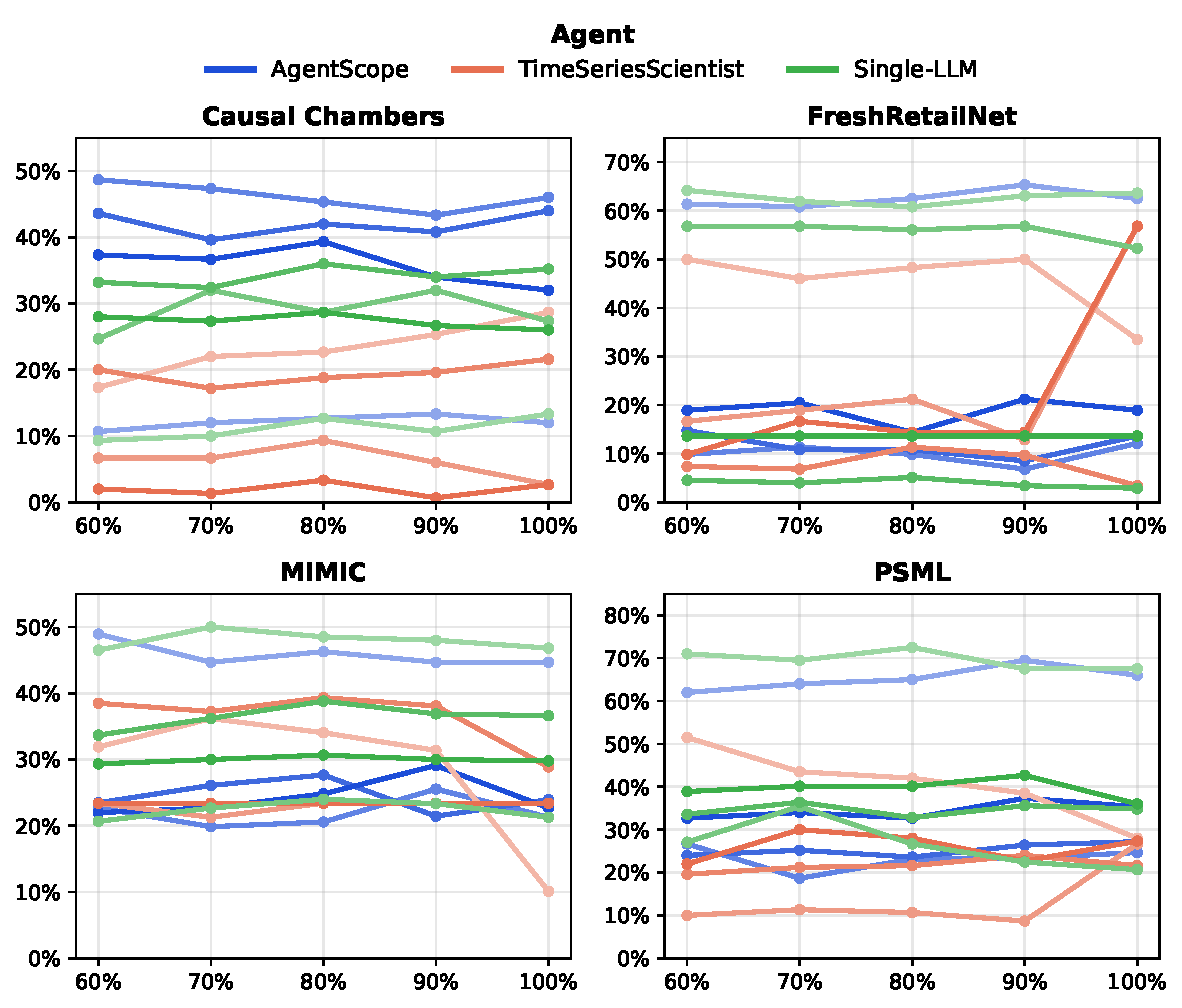
\includegraphics[width=\columnwidth]{images/length_sensitivity_by_dataset.pdf}
\caption{
Effect of input time-series length on agent performance across four datasets.
Each subplot corresponds to a dataset, and multi-choice accuracy is reported for different agents under varying input lengths.
Lines with the same color denote the same agent, while darker to lighter shades represent T1--T4 tasks, respectively.
}

    \label{fig:length_sensitivity_by_dataset}
\end{figure}


Figure~\ref{fig:length_sensitivity_by_dataset} examines how truncating the historical input length affects performance across datasets and task tiers (T1--T4) for three representative settings: a general-purpose agent (AgentScope), a time-series agent (TimeSeriesScientist), and a single-LLM baseline.
A central observation is that history length is not a universally monotonic driver of performance.
Instead, its impact varies substantially across domains and task tiers, and in several cases longer inputs introduce instability rather than consistent gains.

\paragraph{Dataset-dependent sensitivity is substantial.}
The four datasets exhibit clearly different responses to increasing history length.
On PSML, performance curves for AgentScope and the single-LLM baseline are comparatively stable and often improve mildly as more historical context is provided, particularly for simpler tasks such as T1.
This behavior suggests that PSML contains strong recurring temporal patterns that remain exploitable under straightforward truncation schemes.
In contrast, FreshRetailNet shows much weaker and more irregular sensitivity to history length.
For both AgentScope and the single-LLM baseline, most task tiers fluctuate within a narrow range as the input window grows, indicating that additional historical points do not reliably reveal new predictive evidence in the retail setting.
MIMIC exhibits the clearest signs of length-induced instability.
While moderate extensions of the history can be beneficial, very long inputs sometimes lead to sharp performance degradation, most noticeably for the hardest task tier.
This pattern suggests that longer clinical histories may introduce noise or confounding factors that are difficult for LLM-driven pipelines to compress and utilize effectively.
Causal Chambers displays more consistent trends than retail and MIMIC, although absolute performance still varies substantially across tiers, indicating that domain structure rather than raw context length primarily governs difficulty.

\paragraph{Task-tier effects reveal diminishing returns and occasional reversals.}
Across datasets, T1 is the task tier that benefits most consistently from longer historical context.
Even there, improvements tend to saturate once a substantial portion of the history is included, rather than continuing to increase at the maximum input length.
This saturation effect is particularly evident for AgentScope, where the best T1 performance often appears at intermediate-to-long histories.
For prediction- and decision-oriented tasks such as T2 and T4, the trends are noticeably less stable.
Additional history can yield modest gains at moderate lengths, but these gains rarely translate into steady improvements, and in several cases performance reverses when the longest input is used.
This behavior aligns with an earlier observation: these tasks are constrained not only by access to temporal evidence, but also by the agent’s ability to extract the most relevant signals and to maintain controllable, structured outputs as the prompt grows longer.

\paragraph{Differences across agent types highlight distinct failure modes.}
AgentScope, representing a general-purpose agent, tends to be robust yet relatively insensitive to history length.
Its performance curves typically change only modestly as more context is added, especially on FreshRetailNet, suggesting that longer raw histories are not automatically converted into stronger temporal reasoning.
The single-LLM baseline shows a clearer sweet-spot behavior.
Moderate input lengths often match or outperform both shorter and longer settings, while the longest histories sometimes degrade performance.
This pattern reflects a trade-off between contextual richness and controllability, as longer prompts increase the likelihood of drift, constraint violations, or dilution of salient signals.
TimeSeriesScientist exhibits a different and more bimodal response.
In certain domain–tier combinations it can effectively exploit longer histories, most strikingly on FreshRetailNet where a sharp improvement appears at the longest input for one task tier.
At the same time, it is more prone to abrupt drops in other settings, such as a severe degradation at the longest history on MIMIC for a difficult tier.
This behavior suggests that time-series–specific tooling can enable stronger utilization when additional history contains relevant structure, but the pipeline becomes brittle when long contexts introduce heterogeneous regimes or when long sequences are not compressed into stable intermediate representations.

\paragraph{Implications for agent design and benchmark use.}
Two practical implications follow from these observations.
First, longer history should not be equated with better context.
For several dataset and task combinations, extending the input window beyond a moderate length leads to diminishing returns or even reversals, implying that benchmark evaluations should not assume that more tokens confer an inherent advantage.
Second, the results motivate length-aware agent designs.
Rather than relying solely on truncation, agents should incorporate explicit mechanisms for history selection and summarization, such as retrieving the most relevant subsequences, compressing temporal regimes, or extracting structured evidence, in order to prevent long-input dilution and instability.
From a benchmarking perspective, reporting performance at multiple history lengths is essential.
Doing so reveals whether a method genuinely leverages extended temporal evidence or merely relies on short-horizon heuristics, and the strong dataset-dependent sensitivity observed here shows that conclusions drawn from a single fixed length can be misleading.

Overall, the length study underscores that temporal benchmarks should evaluate not only forecasting and reasoning accuracy, but also the ability to robustly utilize additional historical evidence under realistic prompt-length and control constraints.
This capability remains only partially and inconsistently developed across current general agents, time-series agents, and single-LLM baselines.


\begin{insightbox}
\textbf{Insight.}
The ability to utilize longer historical context is itself a fragile and task-dependent capability. Performance saturation and degradation at extended input lengths indicate that temporal reasoning is constrained not only by access to evidence, but by an agent’s ability to select, compress, and control relevant temporal information.
\end{insightbox}


